\documentclass[10pt,twocolumn,twoside]{opticajnl}
\journal{opticajournal} % use for journal or Optica Open submissions

% See template introduction for guidance on setting shortarticle option
\setboolean{shortarticle}{true}
% true = letter/tutorial
% false = research/review article

% ONLY applicable for journal submission shortarticle types:
% When \setboolean{shortarticle}{true}
% then \setboolean{memo}{true} will print "Memorandum" on title page header
% Otherwise header will remain as "Letter"
% \setboolean{memo}{true}

\usepackage{lineno}
\linenumbers % Turn off line numbering for Optica Open preprint submissions.

\title{GeoVis: an interactive map to visualize common climate indicators}

\author[1,2]{Muhammad Alafifi}
\author[1,3]{Jiawei Wu}

\affil[1]{Computer Science Department, Rensselaer Polytechnic Institute, 1999 Burdett Ave, Troy NY, 12180}

\affil[2]{email: alafim@rpi.edu}
\affil[3]{email: wuj22@rpi.edu}

\begin{abstract}
    Geovis is a map rendering of the United States that aims to provide 
    climate enthusiasts or curious individuals with an interactive webpage 
    to visualize common climate indicators such as wind speed, precipitation, 
    and temperature. With the increase in greenhouse gas emissions around the world, 
    it is crucial to visualize such trends that leverages ones understand in climate 
    change. To compile this project, we utilized datasets from \href{https://www.kaggle.com/datasets}{Kaggle} and NOAA (ref).
    Our visualization garnered much important feedback, with many feedback being appreciative of our minimalistic and intuitive design. 
    We found that many testers were curious at our web application because they were found to 
    be clicking on multiple things for the sake of visualizing the data.
\end{abstract}

\setboolean{displaycopyright}{false} % Do not include copyright or licensing information in submission.

\begin{document}

\maketitle

\section{Introduction and Background}

We are both climate enthusiasts, which is why we decided to pursue a 
project that was closely related to visualizing climate. Our intention 
of creating this project was to provide a platform for individuals to 
visualize common climate indicators such as wind speed, precipitation, 
and temperature. We believe that with the increase in greenhouse gas 
emissions around the world, it is crucial to visualize such trends that 
leverages ones understand in climate change. Creating a map visualization 
was what we believed to be the most intuitive way to visualize data, we were 
inspired by wind fm \cite{a2019_wind} and \cite{beccario_2019_earth} earth nullschool.
These sites provide the user with great flexibility in 
manipulating and showing specific climate indicators, something that we took 
inspiration in creating our own.

\section{Data Collection}

To compile this project, we primarily utilized datasets of type csv. 
There are two types of data that we had to process, one is for every 
airport, and another for every county.

\subsection{Airport Data}

Utilizing airports was the most intuitive way to gather weather data. Initially we had planned to use large global datasets, such as NOAA ICOADS \cite{noaa_2017_noaa}, but we found it expensive, given the size of the dataset being 31 million rows and 75 columns. Not only that, but the points that were collected over the United States were so abundant, that it was difficult to visualize and also hindered our efforts to make it interactive. Instead, we pivoted over to a dataset that was more manageable, which was the weather data for 265 airports in the United States \cite{nanduri_2021_weather}. This dataset was much more manageable, with 265 airports. Airports resembled a cleaner visualization as well, as some states have at most 3 major airports, making it simple to visualize the difference.

\textbf{Processing the data} was by no means simple. There wasn't a dataset that was "perfect" for our project, so we had to look for multiple datasets. The datasets we found was always missing some key features. Our airport weather data, while it was useful in providing us with the weather data, it was missing the latitude and longitude of the airports. We had to find another \cite{alaswad_2021_us} dataset that provided us with the latitude and longitude of the airports. We had to merge these two datasets together to create a dataset that had both the weather data and the latitude and longitude of the airports. However, it would be simple if we could just merge the two datasets together to create one, but we ran into one problem. The airport dataset providing us with climate information contained only 265 airports, while our other dataset contained over 3375 datapoints, which are all the airports in the United States.

Our final dataset came out to contain the following columns: \textbf{Month, Day, Temperature (F), Dew Point (F), Humidity (\%), Wind Speed (mph), Pressure (in), Precipitation (in), IATA code, Name of airport, Longitude, Latitude}. With all this data, we were able to begin creating our intended visualization.

\subsection{County Data}

On top of point by point data for major cities and regions, we desired to have a filled or colored in map of the weather data over time. The goal was to have a climate statistics map as a user could easily recognize from weather channels. Initially, we were also looking at the NOAA's NOMADS \cite{noaa_nomads} data set, which contained point data as accurate as a quarter of a degree of longitude and latitude, but several issues arose. Given the data was broken down by every 6 hours and by different levels of altitude, it gave way to issues regarding compiling time and location values. However, more presciently, we ran into the difficulty of formatting the data from the raw GRIB2 (Gridded Binary) format, which is used by the national departments to compactly plot weather data, to a usable CSV or JSON file format, which would have required a lot more time building a constant data translator and using more unused languages/softwares for us such as Perl. Instead, we chose to use county data, as city data won't be as complete, to represent the map data.

Working with county data would be much more manageable given the limited amount of data, given there are $3,143$ counties in the United States. The NCEI \cite{noaa_2019_national} contained appropriate CSV county data sets broken up by month and state, primarily the lower 48, which contained different types of weather statistics from average temperature to precipitation. We chose to use those as the two major map data sets given that they could can be contrasted well on each other and along with the airports' weather parameters. The first measure of business was having to manually download the CSV data for each state. When looking at our map data set and temperature data set, we realized that the map data set used the FIPS county code for its set, so - using python - we compiled the states all together in one file and another python script to convert the counties into a usable FIPS code. Finally, the last issue to deal with that was breaking the data set was county names that contained commas or illegal characters for the csv, this meant manually running through every file and editing them out.

\section {Visualization and Progress}

For our visualization, our intention was to create a map of the United States that allows individuals to be able to access climate data in our chosen airports. 

\subsection{Progress Report 1: Map and Regions Rendering}

Map rendering is a key feature of our project. Rendering a map of the United States allowed us to begin learning the D3 stack and also envision the data that we will need to plot the points onto the map. We use topojson \cite{bostock_2024_topojsontopojson} and follow this D3 guide \cite{d3_2023_us} to create and render our intended US map.

\begin{figure}
    \centering
    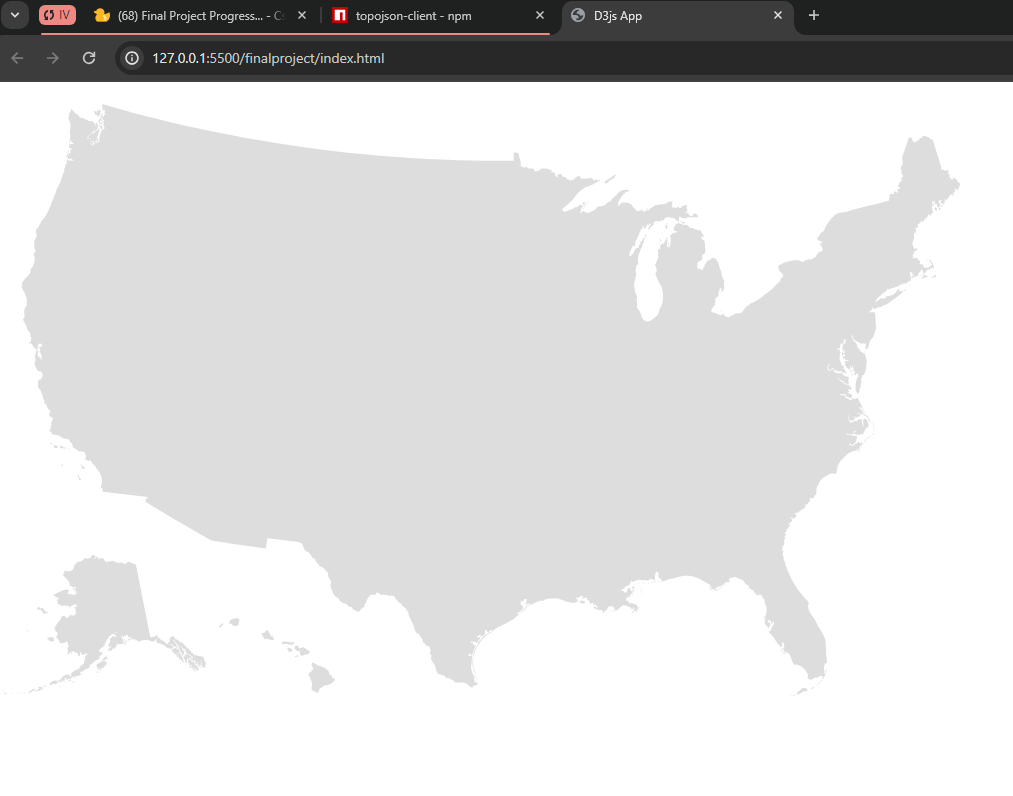
\includegraphics[scale=0.25]{images/img1.png}
    \caption{Our first map rendering of the United States}
\end{figure}

While topojson is our choice, it is not the only way to render a map. We also considered using geojson \cite{mapbox_geojsonio}, but we found that topojson was more efficient in terms of file size, that is to say, they claim that their file sizes are over 80\% smaller than geojson files, as claimed on their \href{https://github.com/topojson/topojson}{Github project description}, and we had difficulties dealing with adjusting and handling visualization in the past. Additionally, after we had decided against using defined point data, we rendered a TopoJSON of the county borders, aligning it on top of the rendered map (figure).

\subsection{Progress Report 2: Plotting the Airports and County Data}

\begin{figure}
    \centering
    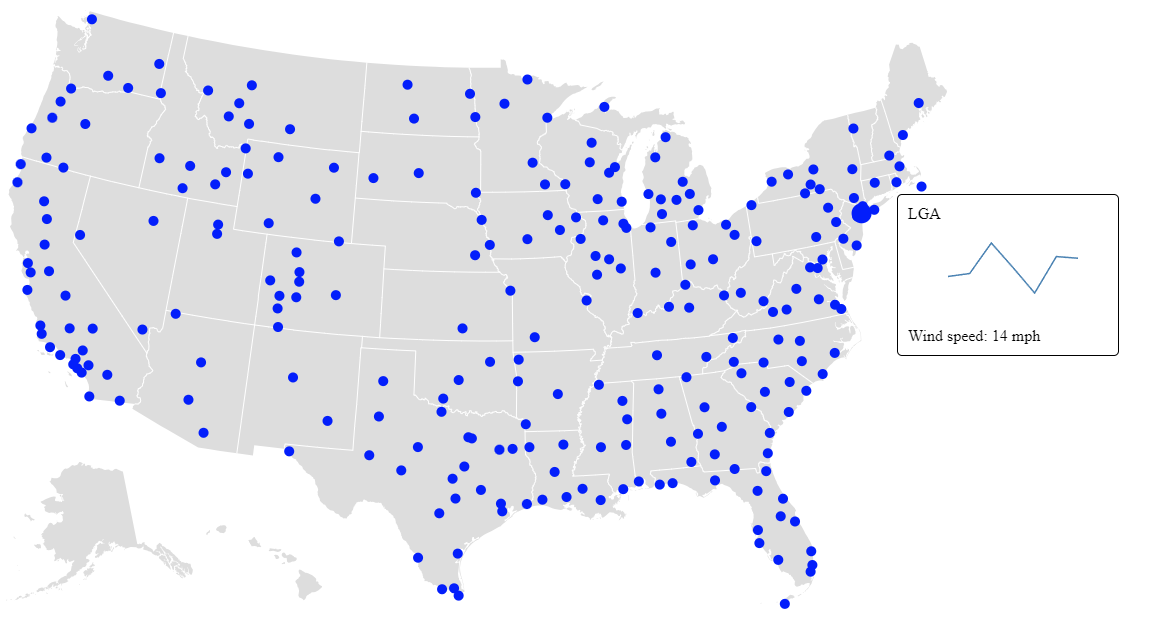
\includegraphics[scale=0.25]{images/img2.png}
    \caption{Plotting the airports on the US map}
\end{figure}

Fig 1 provides us with a starting point to plot the airports. For our dataset, we have information like the latitude and longitude of the airports, which is crucial for plotting them in topojson. Fig 2 shows the 265 airports all plotted out onto our map of the United States. An additional feature that we included was a slight hover effect. Hovering over each airport would enlarge the airport point, this decision was done so that it would be easier for users to see which airport they are hovering over. At this point, if you decide to select on an airport by clicking on it, it would display information about that airport. More specifically, the airport name, the wind speed for that airport, and also a line chart to show the trend of the wind speed over the last 7 days.

While this provides a starting point to what we want to do, there are still many things missing. For example, the line chart that we have included for each point's tooltips was unlabeled, it had no axis, making it difficult for the user to intuitively understand what chart is displaying. Not only that, but the points are all colored blue, which is not very intuitive. We need to color the points based on the climate indicator that we want to display.

Additionally, at this time, we began formatting the data sets to fit into the TopoJSON. (pink figure) demonstrates a test data set built with python that aligns the color strength with the county's coordinates. Once the temperature data for a month was properly formatted, we mapped the values to the county FIPS code, filling in the counties using D3's svg fill feature. (temp initial figure) represents our data set. 

When picking out a color set, we used ColorBrewer (ref) to pick out a color scheme. Considering temperature is often represented as red: hot, blue: cold, we decided to imitate the color choices found on many temperature maps to maintain familiarity, thus we chose a divergent scheme with a shade of red and blue on each end. One thing that came up was whether we use a discrete or linear color spread. We ended up deciding against using a discrete scheme as we found that the discrete theme would feel too disjoint and misrepresent some counties to be too similar. Additionally, a linear scheme would be easily understood, and it would allow us replicate the feeling of a "painted" on weather map, as previous mentioned (see figures).

\subsection {Progress Report 3: Implementing the Time Slider}

\begin{figure}
    \centering
    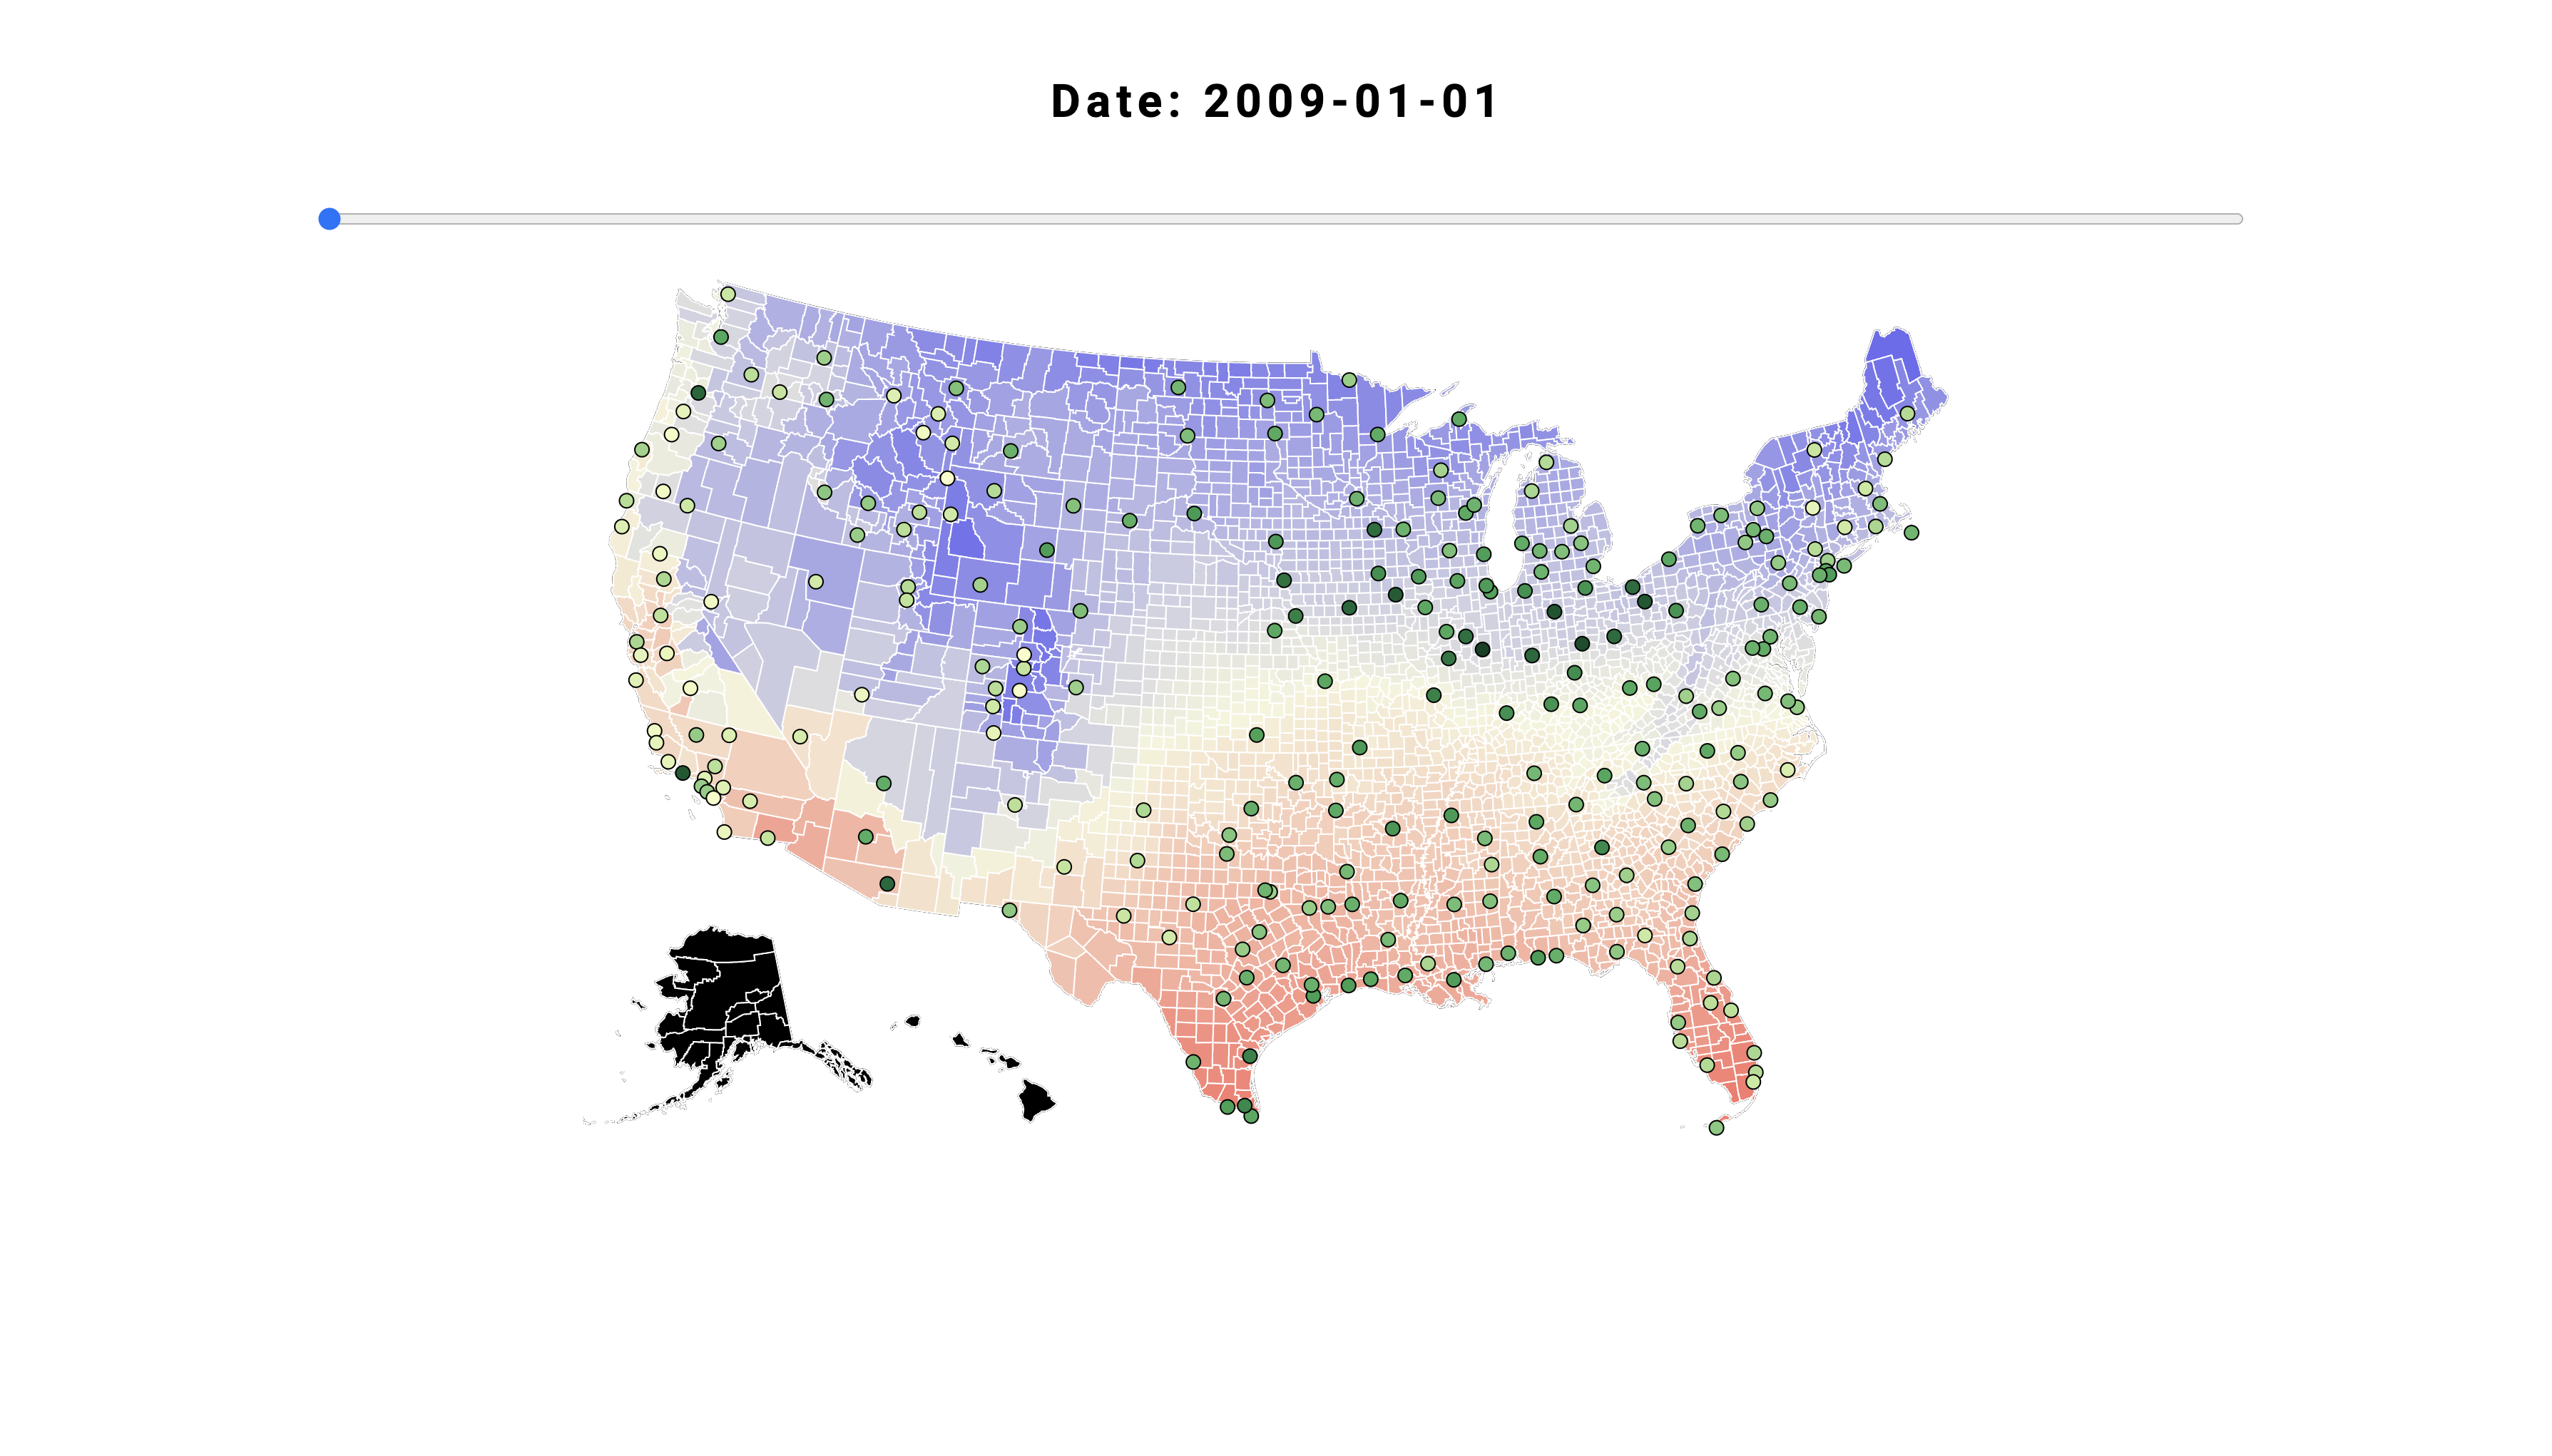
\includegraphics[scale=0.10]{images/img3.png}
    \caption{Implementing the time slider}
\end{figure}

Time slider implementation was a crucial feature that we wanted to implement. We wanted to allow users to be able to select a specific date and see the climate data for that specific date. Fig 3 shows the implementation of the time slider. The time slider allows users to select a specific date, and the points on the map would update to show the climate data for that specific date. This was done on client-side rendering with an event listener.

\begin{algorithm}
    \caption{Time Slider Implementation}
    \begin{algorithmic}[1]
    \Procedure{TimeSlider}{}
    \State $selectedDate \gets sliderValueToDate(this.value)$
    \State $updateDisplayedDate(selectedDate)$
    \State $updateVisualization(selectedDate)$
    \EndProcedure
    \end{algorithmic}
\end{algorithm}

This algorithm is called with a 'onchange' event listener, which is triggered whenever the user changes the value of this slider. To remove excessive rendering, we implemented the slider in a way that it only re-renders when you release the point, not when you move it along the slider. We made this decision because our dataset is about 70mb in total, and re-rendering the data when you slide along 365 days caused some delays and lags in rendering. So rendering it only when you release the point was a good compromise.

\begin{figure}
    \centering
    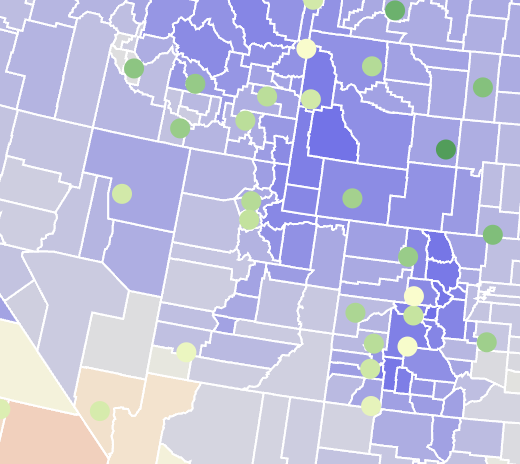
\includegraphics[scale=0.45]{images/img5.png}
    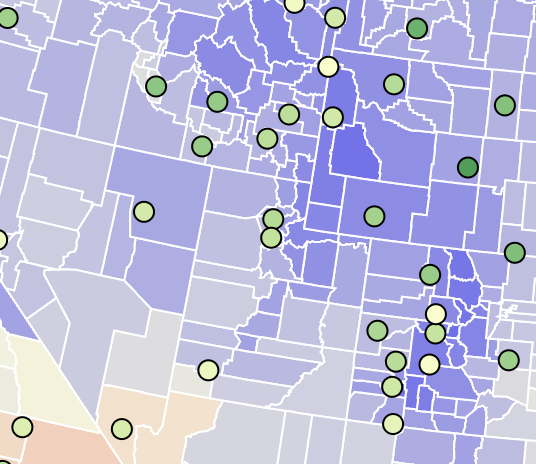
\includegraphics[scale=0.45]{images/img4.png}
    \caption{Color choice on the airports based on wind speed}
\end{figure}

Fig 4 shows the choice made in coloring each airport. We decided to select a sequential green hue coloring for our color representation. On the left side, we have filled the circle with the color respective to their wind speed, however, for the lighter colors such as on the south west side, it became more difficult to distinguish between the point and the background. The choice that we decided to make to fix this issue was by implementing a border. The effects of the border is shown in the right image, which makes it easier to distinguish between the points and the background of the map.

\begin{figure}
    \centering
    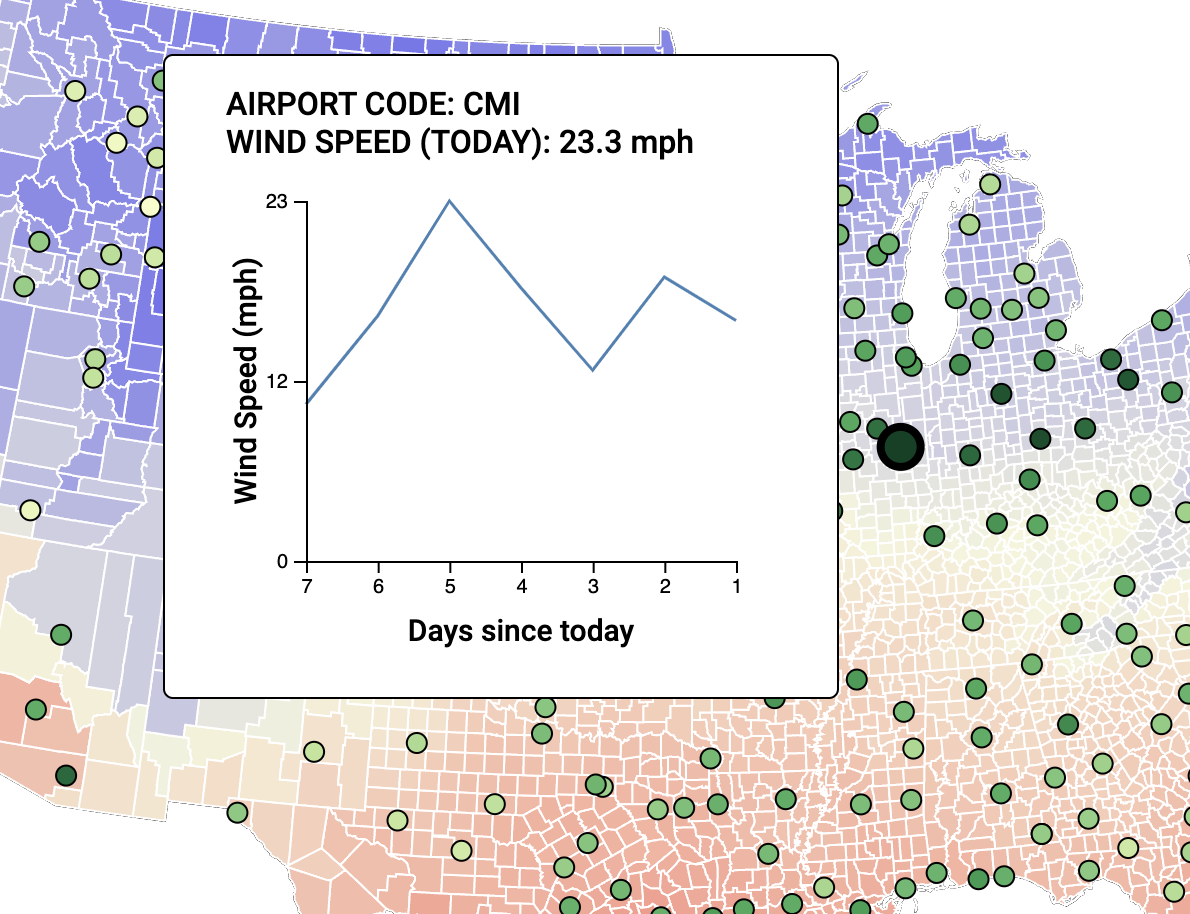
\includegraphics[scale=0.4]{images/img6.png}
    \caption{Tooltip improvements}
\end{figure}

Fig 5 shows the improved tooltip. It shows you the airport IATA code, the wind speed for the day, and also the improvement line chart from progress update 2. Since it was a line chart, we made the decision to flip the x-axis so it would easier to visualize the trend, with the right side being the nearest day, and the left side being the further day.

Using Javascript and D3's 'onchange' feature, we also implemented a change of the type of graph from temperature to precipitation based. This meant now also implementing a method that would change the type of map displayed. For actually displaying the map, we now ran the same scripts - previously used to parse the temperature - on the manually downloaded precipitation data, and used the 'onchange' function to determine which of the two maps to render. This meant that we also had to pick a new color scheme from Colorbrewer (ref). We chose to use a sequential map to represent increasing amounts, and chose a white to green theme, given that green is often associated with cooler themes and since we didn't want to create confusion with the blue from temperature, and white could represent 0, as opposed to all being a single hue of green (figure map). 

\subsection {Final Visualization}

For our final visualization, we included not only a legend for the points, but also a toggle for users to switch between the climate indicators such as temperature, dew point, and wind speed. Fig 6 shows the final implementation. We have the time slider on the top, the legend for the airport on the bottom right, and a stats box that on the bottom left, indicating the highest selected climate indicator for that day, along with the location in which it occurred as shown in Fig 7.

\begin{figure}
    \centering
    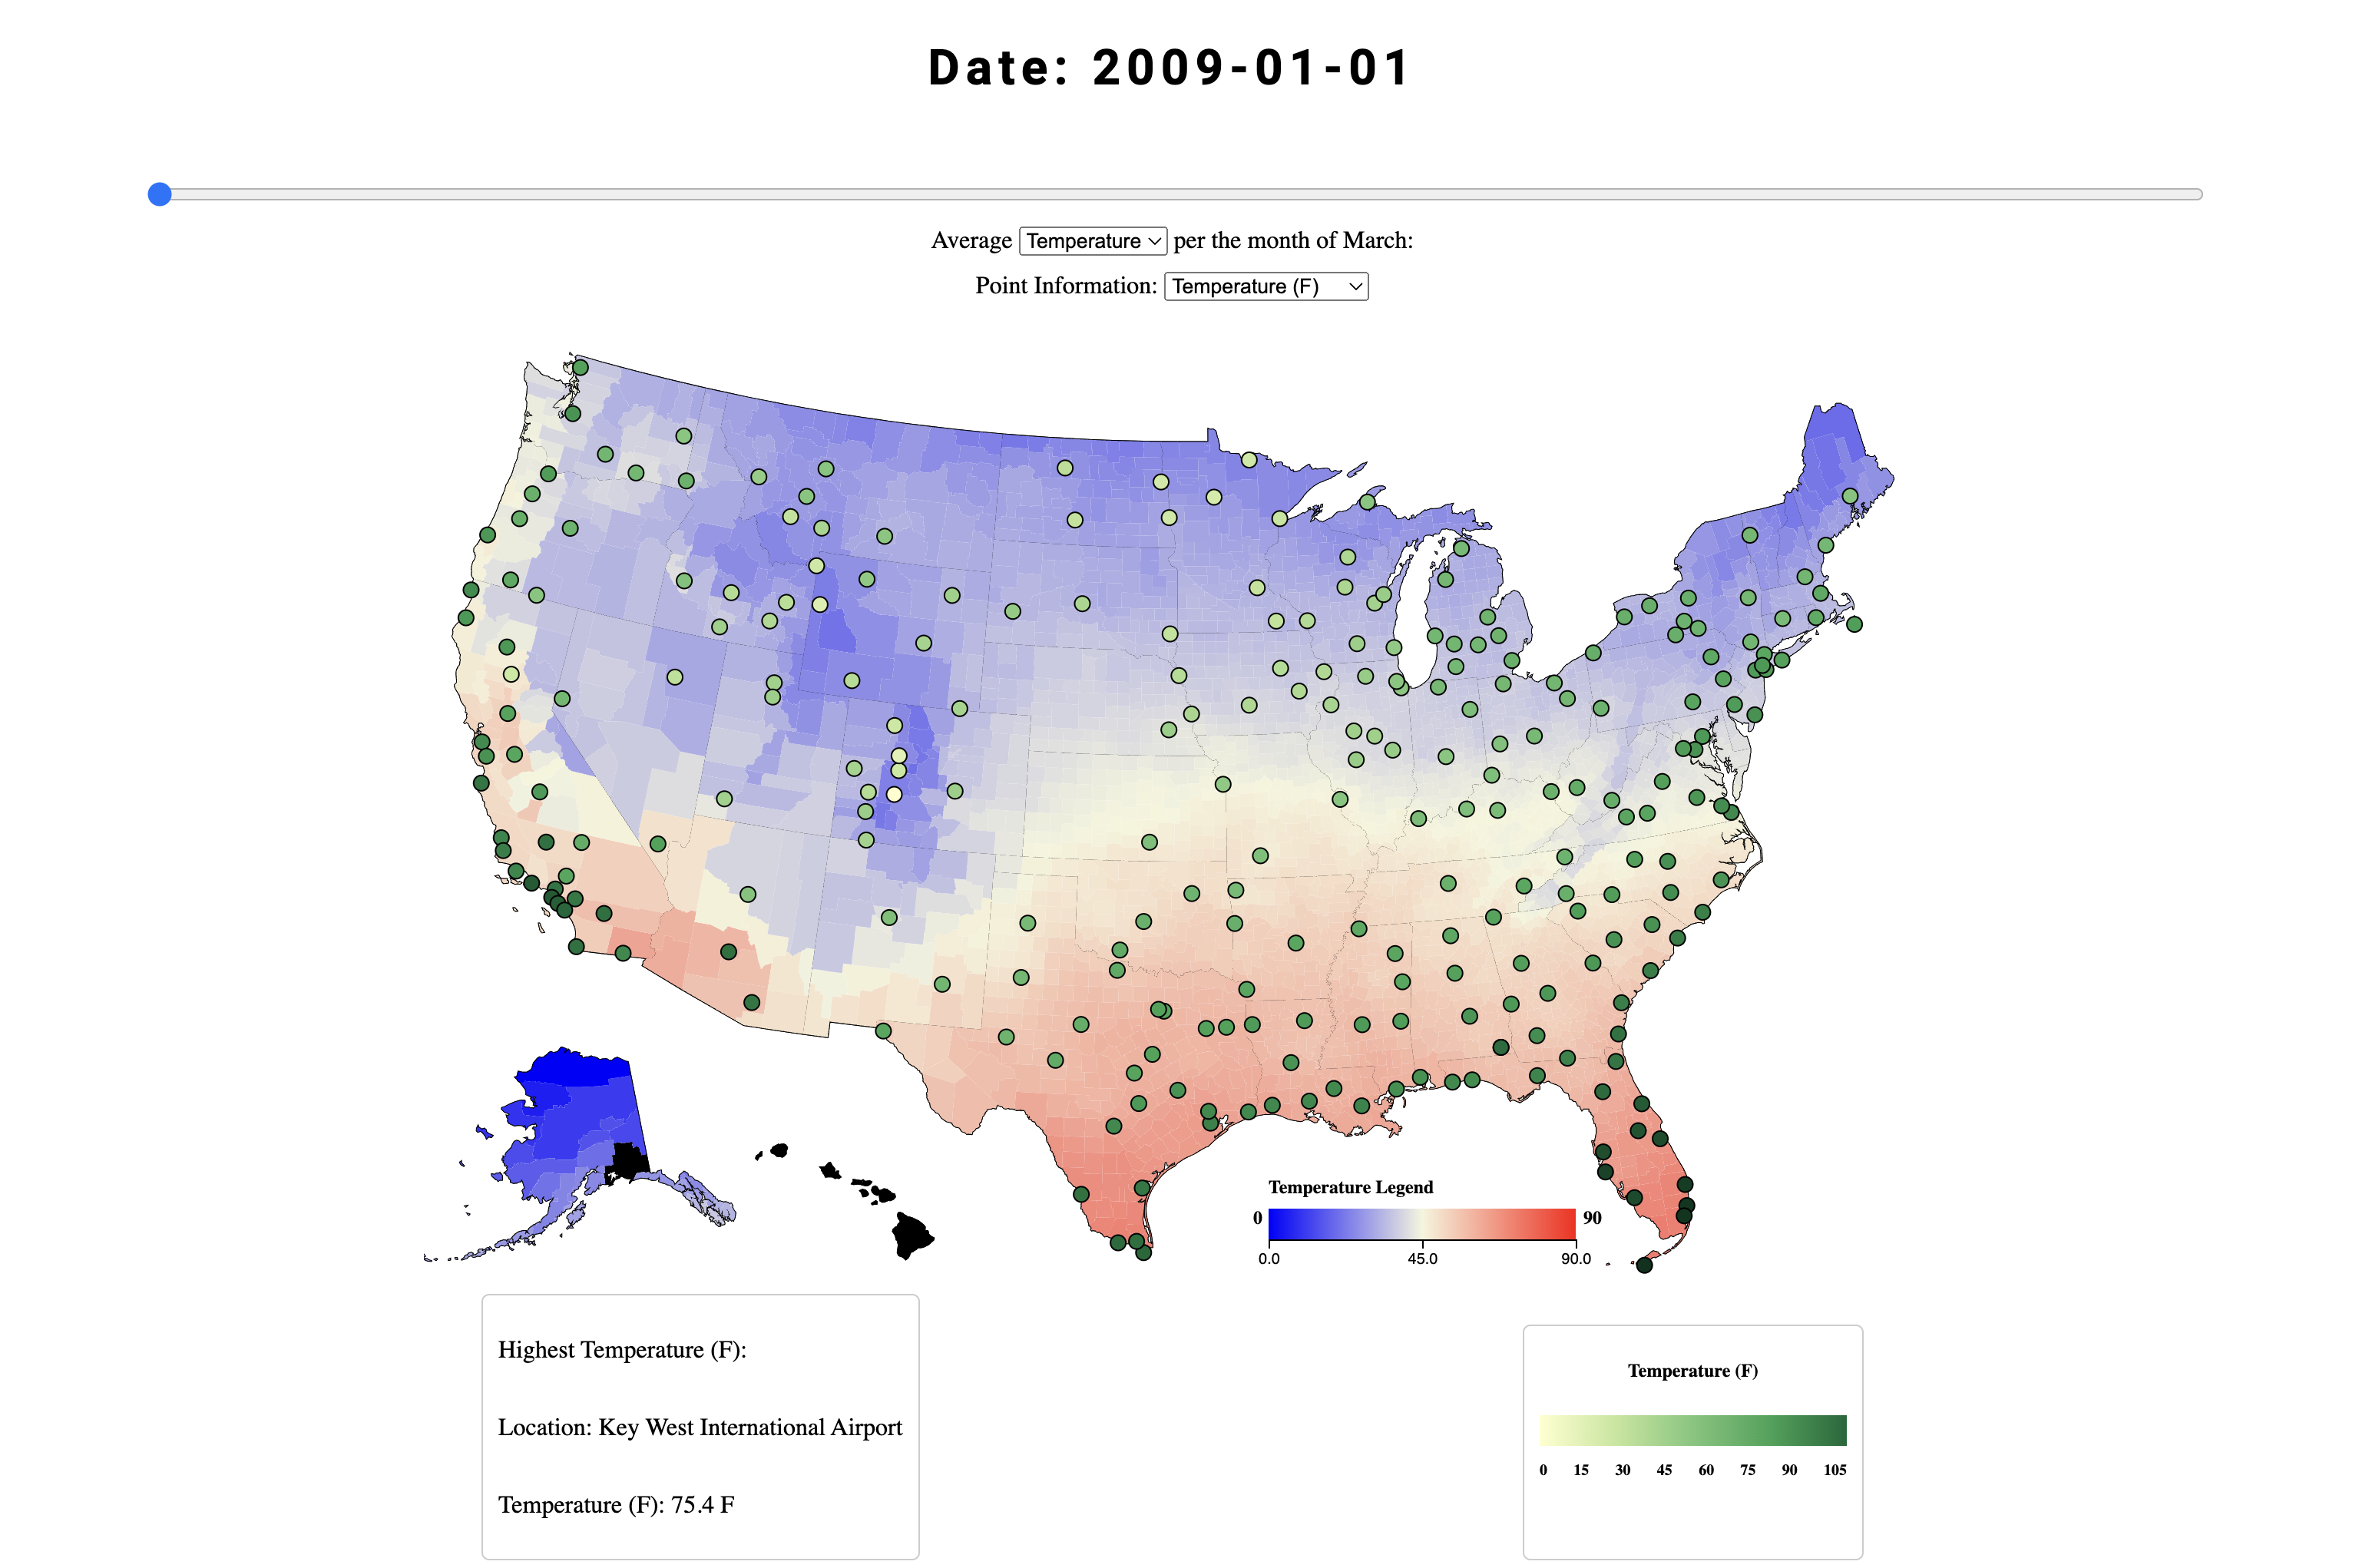
\includegraphics[scale=0.15]{images/img7.png}
    \caption{Final Visualization}

    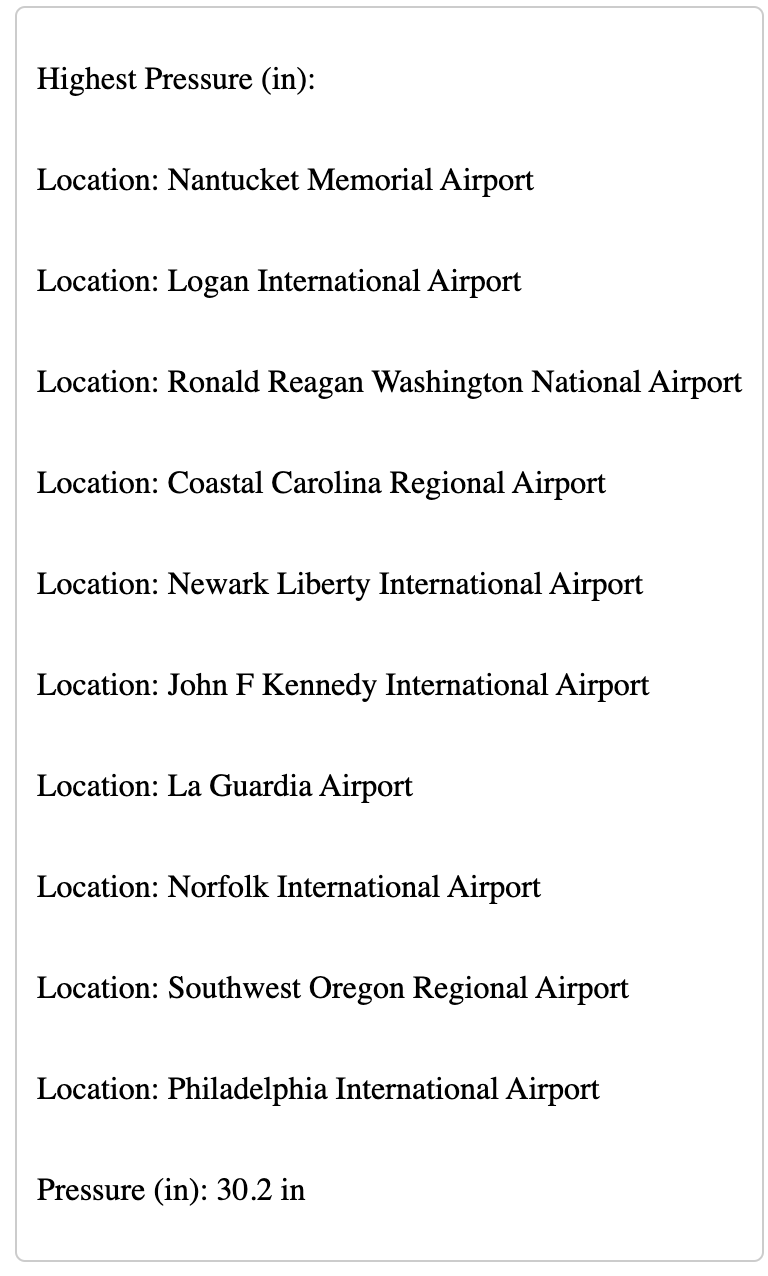
\includegraphics[scale=0.5]{images/img8.png}
    \caption{Multiple Airports have the Highest Pressure for the selected date}
\end{figure}

In addition, one of the crucial improvements that we wanted to implement was the tooltip for each of the airports. Our final tooltip (Fig 8) shows the full name of the airport that you selected. This felt more intutiive in the audience knowing which airport it is, given that airports with an unfamiliar airport code were unknown to users. In addition, since we had data on all the climate indicators, we thought it would also be the best to include statistics on all the weather indicators, and the line chart should only show the climate indicator selected. In Fig 8, temperature was selected as the toggle for Point Information, and the line chart reflects by graphing the temperature data for the past 7 days.

\begin{figure}
    \centering
    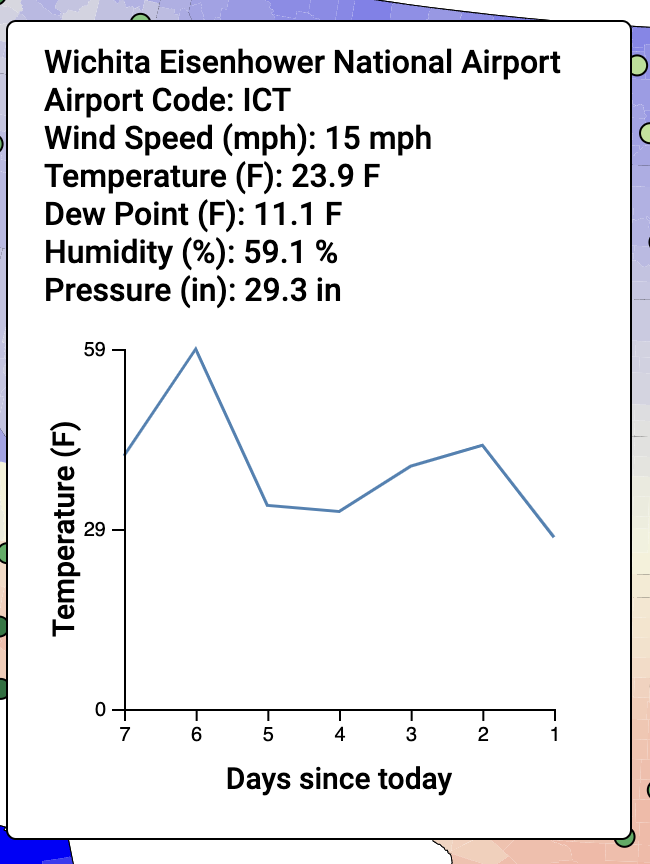
\includegraphics[scale=0.5]{images/img9.png}
    \caption{Final tooltip design}
\end{figure}

\section {Feedback}

\subsection{Muhammad's Feedback}
Going into the feedback section, I wasn't entirely sure what to expect. We had completed most of the important points of usability that we had set for ourselves after initial feedback on the proposal and first couple of weeks. Thus going in, I didn't always ask the same question; however, I was asking about how more information could be added to the visualization, as it felt empty and static outside of time change. 

One of the suggestions was to display the time trends of not just wind data, but all the possible statistics when hovering over cities. Contrarily, I also heard it would have been appreciated had there been a way to switch the airport wind speed data for temperature over the past week, or any other, based on the user's preference. I also received feedback that seeing the recent temperature trends of a county/region/city while looking at the map would be useful. We decided to tackle this by taking the climate data provided in the airport set and creating a user switch between the different climate stats provided. When I asked about how a user would feel about placing indicators of precipitation over the temperature map, some indicated interested; however, the general consensus was that it could distract from the cities/airports and would be more useful as a toggle.

Collectively, however, regarding this question, we heard that adding more map elements would crowd the visualization, thus we decided to implement more changes that gave control to change the visualization to the user.

Some other feedback received was considering how large the data set was. Given that it was plenty of points across a whole year each day with its own weather stats for the airport points, it does take a non-unnoticeable amount of time to refresh. Additionally, loading the data in case any changes were done takes upwards of 15 minutes running. Thus, a suggestion that came up was to break down the data by 7 day segments, thus the graphs could be succinctly kept but the slider much less minute in detail. We discussed but ultimately decided against given that it would disjoint the feeling of the current daily slider. Additionally, breaking up the data would result in an uneven week total, since the number of weeks doesn't divide perfectly. Finally we wanted the user to be able to look at any prospective day and look at the past 6, not just to be stuck looking at the next 6 if it was the last in the set.

Finally, some more feedback that we were able to partially follow through on was based on the color choices used. Primarily, one suggestion was to implement a colorblind friendly mode for the colors, especially considering we're using green on red, and beige next to the red. We switched the temperature coloring to one with more distinct points and ends from colorbrewer's (ref) diverging colorblind safe options. We didn't apply a fully colorblind safe feature, especially for the airport points being green; however, we ensured the point contains distinct black borders to draw it away from blending with the background. Additionally, there was a suggestion regarding the missing or faulty data representations. Currently, if a county has missing or faulty data for a specific time period, it will appear blacked out (see image), which could cause confusion with high precipitation levels for example. When I asked what could be better done to represent the data, it was brought up to use a pattern - such as diagonally stripped or spotted - in the county. As indicated, that is something we didn't implement, as during testing there were initially difficulities, and in later stages, it seemed like the approaches would create too much clutter, but is spoken further in \textit{Future Work}.

\subsection{Jiawei's Feedback}
I was fortunate enough to receive a lot of useful feedback. My question during the feedback process was to ask about what should be placed in the blank spaces in the webpage, as the left and right sides were mostly empty and we could implement some sort of left and right rail to fill up to gaps. Our most common feedback was to implement a stats box that allows the user to view some of the highest climate indicators for that day. I thought this was a great idea, which is why we implemented this into our application for the final version.

A legend for the wind speed was also important, many users were confused about what the colors of the points represented, some of them believed the colors are indications of how "large" an airport is, with darker colors meaning a larger airport, and lighter colors meaning a smaller airport. This was a great suggestion, and we implemented this by adding a legend for our points.

Another suggestion was to add a toggle for the climate indicators. Some people may not only be interested in wind speed, but also other types of climate indicators. This was a great suggestion, mostly because we already had the data for other climate indicators, so it would be simple to implement it onto our application. We went with a toggle version to select different climate indicators. To do so, we needed to improve our python script to include the other climate indicators and create a new final dataset that includes all the climate indicators along with their respective values. 

\textbf{We were not able to implement all the feedback that we received.} One of the important feedbacks that we got was to find a way to color the points to represent which airport is classified as a "large airport" and "medium airport". Since we are using colors of the points to represent the values for the chosen climate indicator, it was difficult to find a common ground on trying to represent the size of the airport. Some of the thoughts that we considered was making it a different shape, perhaps large airports would be a triangle instead of a circle. But this was never added to our final visualization.

\textbf{Another feedback} that we attempted to implement was a comparison between dates. Users could select a specific date, and then select another date, and the points would update to show the difference between the two dates. This was a great suggestion, but we were not able to implement this feature due to time constraints and also difficult bugs that we struggled to fix, so it never made it to our final visualization.

\section {Challenges}

\textbf{Data collection} was definitely one of the more significant barriers to our success. We struggled with finding a dataset with all the information that we needed, so we ended up having to combine different datasets for the airport data.

\textbf{Stack} also posed a challenge for us. We were not familiar with the D3 stack, and we had to rely heavily on trying to map the examples given on the D3 gallery \cite{d3_2020_gallery} to our own project.

\textbf{Time} was also a significant challenge. Our initial proposal was a similar idea, but we wanted to apply it globally. We would first render a map of the entire globe with scrolling and zooming in features, and then plot the points as seen in the United States map. However, we quickly realized that the data collection was going to be exponentially more difficult and time-consuming. We struggled to find the data that we needed. We later realized after a week that this was not going to be feasible given the time that we had, so we pivoted to a more manageable dataset and focused instead on the United States.

\section {Work Distribution}

\subsection {Muhammad Alafifi}
\textbf{For our visualization}, Muhammad was responsible for gathering and processing all the datasets relating to the refined climate trends across the scope of the project. He also was responsible for gathering the TopoJSON data set for the map which contained the county borders and data to be ID. He was responsible for also finding the most appropriate and reliable/usable data set for the counties, once it was decided that we were breaking down the map into a choropleth of counties. Thus Muhammad also worked on formatting the TopoJSON to fit on the old US region map and formatting the county weather data set so that it could be mapped towards upon the map. Additionally, Muhammad was responsible for making the transitions between types of choropleths renderings, which included the interface.

\subsection {Jiawei Wu}

\textbf{For our visualization}, I was responsible for gathering and processing all the datasets relating to the airports as well as the climate data on each airport. I was responsible for implementing the time slider and its functionalities, creating the rendering of the US map, plotting the airports in their respective location, selecting colors for their respective climate indicators, and creating the pop-up window that shows the climate data of each airport. I was also responsible for creating the legend that shows the range of values for each climate indicator. In addition, I also implemented a selection for the climate indicators for the airport points for users to switch between temperature, dew point, wind speed, humidity, and air pressure.

\textbf{For our project write up}, I was responsible for writing the abstract, [1] introduction and background, [2a] data collection for the airport data. I was responsible for writing the progress report for anything relating to aiport data and visualization with the points.

\section {Citations}

% \bibliographystyle{plain}
\bibliography{iv}

\end{document}
